\section{Results}
\label{sec:results}

All results are on the held-out test period, the final 15\% of the sample: 271 trading days across 20 companies (5{,}420 predictions). Neural configurations report mean $\pm$ standard deviation over seeds 42, 123 and 456. The test set was evaluated once per configuration, after checkpoint selection on validation.

\subsection{Forecasting performance}

\begin{table}[H]
\centering
\input{tables/main_results}
\caption{Test-set performance. MAE and RMSE are in log-return units scaled by $10^{3}$, so $20.869$ corresponds to an MAE of $0.020869$; model differences fall in the third decimal place at this scale. Values are mean $\pm$ standard deviation over three seeds, except for the deterministic rows (the naive references and VAR), which are run once. Directional accuracy is undefined for the zero forecast, which makes no directional call. IC is the pooled correlation between predictions and outcomes.}
\label{tab:main}
\end{table}

\begin{figure}[H]
\centering
\includegraphics[width=\textwidth]{figures/metric_comparison.png}
\caption{Test MAE (left) and directional accuracy (right). Grey bars are naive references; the red line marks chance-level direction. Every model clusters within $0.0004$ MAE of the zero forecast, and every directional accuracy falls within 3.3 percentage points of chance.}
\label{fig:metrics}
\end{figure}

Three observations follow directly from Table~\ref{tab:main}.

First, \textbf{no model beats the zero forecast}. The zero forecast attains MAE $0.020869$. The best graph model, MTGNN with a learned graph, attains $0.020948 \pm 0.000018$, which is \emph{worse}. The seed-to-seed standard deviation of each neural configuration ($1.5$--$4.4 \times 10^{-5}$) is the same order of magnitude as the gaps between configurations, so the ordering among them is not resolvable.

Second, \textbf{the apparent leader is a constant}. VAR attains the lowest MAE ($0.020820$) and the highest directional accuracy ($0.5332$). However, AIC selected \emph{zero} lags on the training window, reducing VAR to a per-company intercept. Its predictions are bit-identical to the train-mean drift forecast: the maximum absolute difference between the two prediction matrices is exactly $0.0$, and both are constant over time. VAR's directional accuracy therefore measures only the fraction of test days on which a company's return shared the sign of its training-period mean, which is the equity drift. It reflects no conditional forecasting.

Third, \textbf{the models predicting at realistic scale perform worst}. Persistence is the only method whose prediction dispersion matches the target (Section~\ref{sec:shrinkage}), and its MAE is $0.030525$, some 46\% worse than the zero forecast. LSTM, the second-least-shrunken model, is the worst trained model at $0.021167 \pm 0.000044$.

\subsection{Statistical significance}

Because the differences in Table~\ref{tab:main} are small relative to their variability, we test them with Diebold-Mariano tests on daily mean absolute loss differentials, using a Newey-West HAC variance estimate \parencite{diebold1995comparing}.

\begin{table}[H]
\centering
\begin{tabular}{lccl}
\toprule
Model & DM statistic & $p$-value & Verdict vs.\ zero forecast \\
\midrule
VAR / Train-mean      & $-1.873$  & $0.061$   & no significant difference \\
MTGNN (learned)       & $+0.384$  & $0.701$   & no significant difference \\
CMA-ES                & $+0.465$  & $0.642$   & no significant difference \\
MTGNN (correlation)   & $+0.834$  & $0.405$   & no significant difference \\
MTGNN (identity)      & $+1.374$  & $0.170$   & no significant difference \\
LSTM                  & $+3.309$  & $0.0009$  & \textbf{significantly worse} \\
Persistence           & $+18.101$ & $<0.0001$ & \textbf{significantly worse} \\
\bottomrule
\end{tabular}
\caption{Diebold-Mariano tests against the zero forecast. A positive statistic means higher loss than the reference. Only two of fourteen comparisons reach the 5\% level, and in both the model is significantly \emph{worse} than predicting zero.}
\label{tab:dm}
\end{table}

Not one model is significantly better than predicting zero. The closest is VAR at $p = 0.061$, and VAR is the constant forecast. Pairwise tests among the graph variants are uniformly non-significant: learned vs.\ correlation $p = 0.49$, learned vs.\ identity $p = 0.26$, learned vs.\ CMA-ES $p = 0.85$, correlation vs.\ CMA-ES $p = 0.48$.

\subsection{Shrinkage: why the error metrics order as they do}
\label{sec:shrinkage}

\begin{table}[H]
\centering
\begin{tabular}{lccccc}
\toprule
Model & std(pred)/std(target) & MAE & Daily IC & 95\% CI & Slope \\
\midrule
Zero forecast        & $0.000$ & $0.020869$ & ---       & ---                & --- \\
VAR / Train-mean     & $0.024$ & $0.020820$ & $+0.0289$ & $[-0.018, +0.076]$ & $0.86$ \\
MTGNN (correlation)  & $0.048$ & $0.020894$ & $-0.0104$ & $[-0.056, +0.035]$ & $-0.37$ \\
CMA-ES               & $0.053$ & $0.020885$ & $-0.0078$ & $[-0.049, +0.034]$ & $-0.14$ \\
MTGNN (learned)      & $0.055$ & $0.020884$ & $-0.0081$ & $[-0.050, +0.034]$ & $-0.05$ \\
MTGNN (identity)     & $0.060$ & $0.020911$ & $-0.0158$ & $[-0.057, +0.026]$ & $-0.09$ \\
LSTM                 & $0.183$ & $0.021155$ & $-0.0285$ & $[-0.069, +0.013]$ & $+0.03$ \\
Persistence          & $1.000$ & $0.030525$ & $+0.0062$ & $[-0.038, +0.050]$ & $-0.02$ \\
\bottomrule
\end{tabular}
\caption{Prediction dispersion, error and signal content, ordered by dispersion ratio. The target standard deviation is $0.030938$. ``Slope'' is the regression coefficient of realised on predicted return; a calibrated forecast has slope $1$. Every IC confidence interval contains zero.}
\label{tab:shrink}
\end{table}

\begin{figure}[H]
\centering
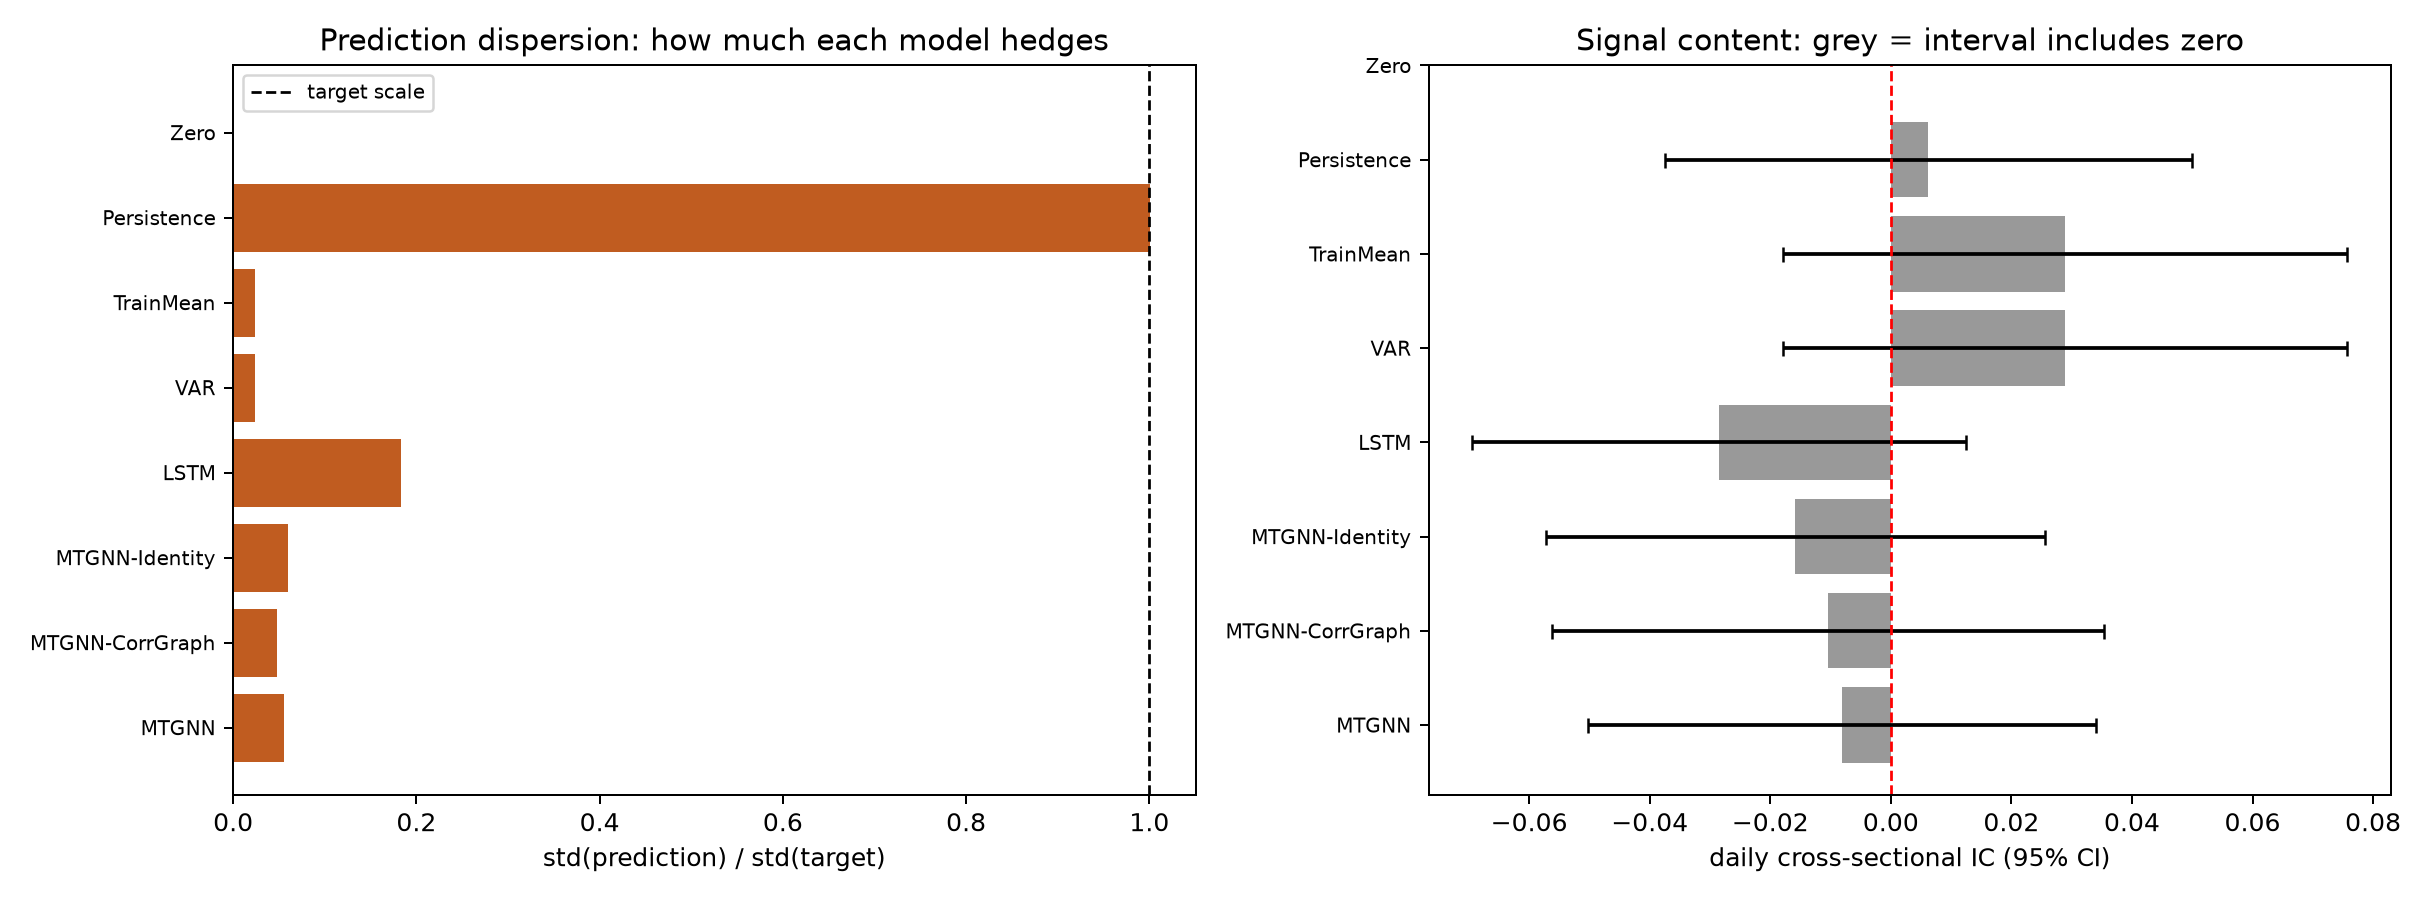
\includegraphics[width=\textwidth]{figures/shrinkage_and_ic.png}
\caption{Left: prediction dispersion relative to the target. Every trained model collapses to between 2\% and 18\% of the target's scale. Right: daily cross-sectional IC with 95\% intervals; grey indicates an interval containing zero, which is the case for every model.}
\label{fig:shrink}
\end{figure}

The ordering in Table~\ref{tab:shrink} is close to monotonic and runs opposite to intuition: \textbf{the more a model shrinks its predictions, the lower its MAE}. The extremes make this unambiguous. The zero forecast has dispersion ratio $0.000$ and MAE $0.020869$; persistence has ratio $1.000$ and MAE $0.030525$. Every trained model sits near the shrunken end, between $0.048$ and $0.183$. Figure~\ref{fig:pred} shows the same effect in the raw predictions.

\begin{figure}[H]
\centering
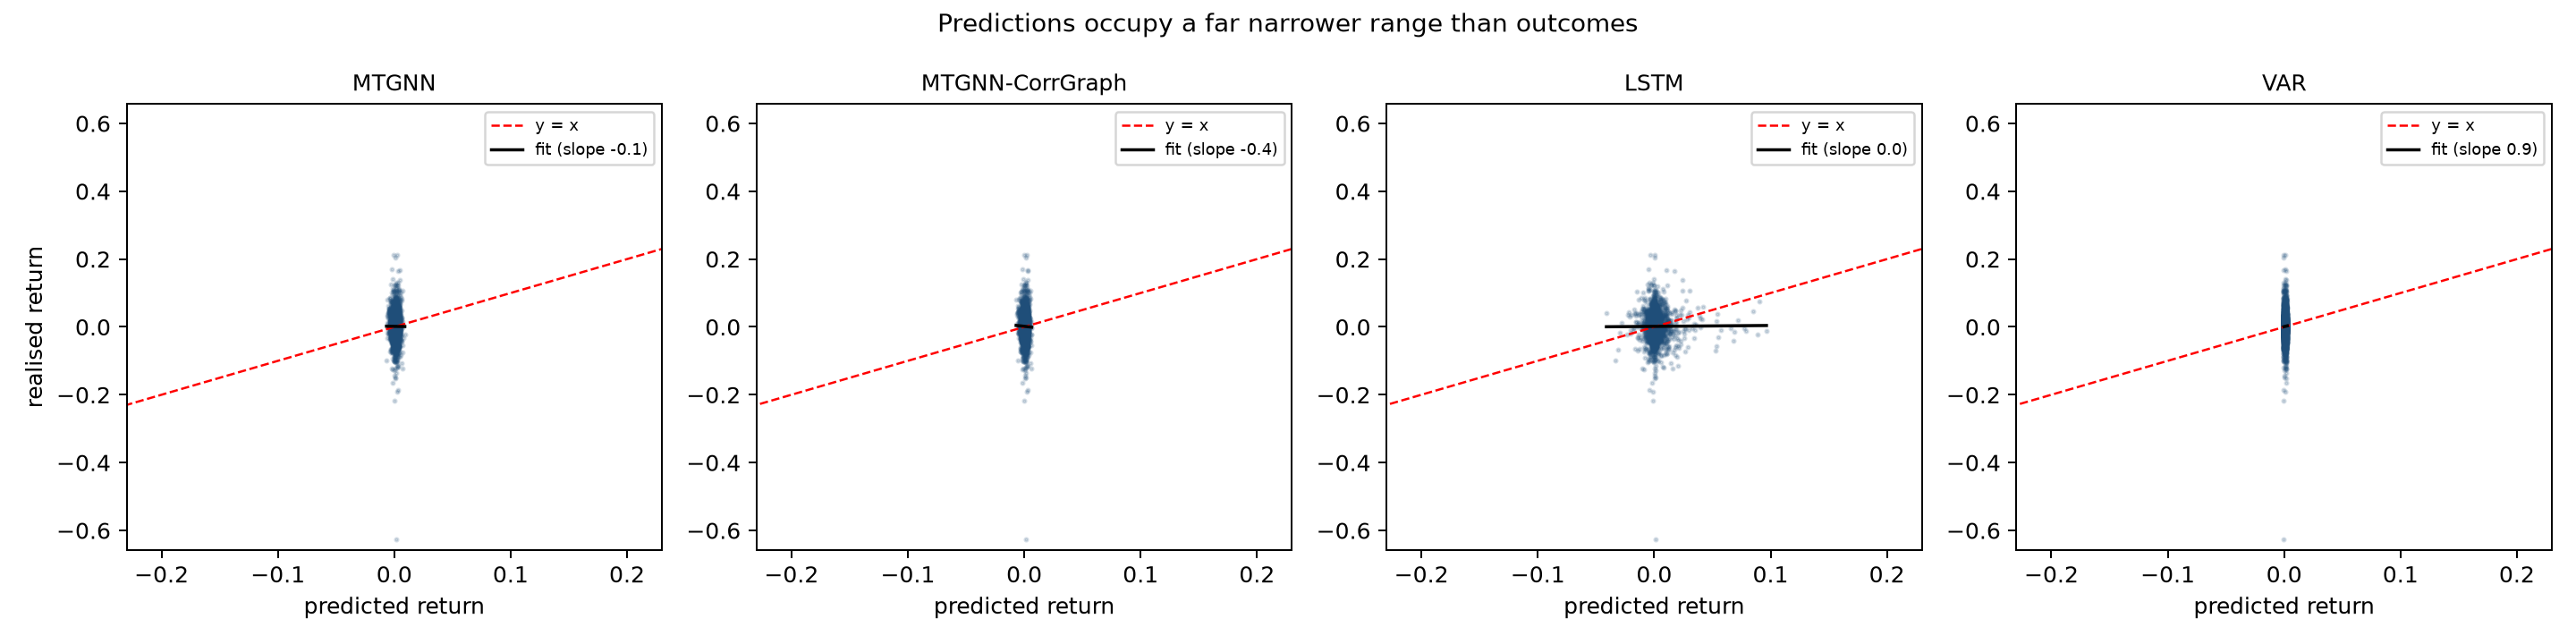
\includegraphics[width=\textwidth]{figures/pred_vs_actual.png}
\caption{Predicted against realised returns. The $x$-axis spans roughly one third of the $y$-axis range: predictions occupy a far narrower band than outcomes. Fitted slopes are near zero or negative, indicating no usable linear relationship.}
\label{fig:pred}
\end{figure}

No model's IC interval excludes zero, including VAR's ($+0.0289$, $[-0.018, +0.076]$). We compute the interval over days rather than over all day-company pairs because same-day returns share a common market factor; pooling all 5{,}420 pairs as independent would understate the interval by roughly $\sqrt{20}$ and make these noise-level ICs appear significant.

\subsection{Ablation: the contribution of the learned graph}

Four variants share one backbone and differ only in the adjacency matrix.

\begin{center}
\begin{tabular}{lc}
\toprule
Adjacency & Test MAE \\
\midrule
Identity (message passing disabled) & $0.020940 \pm 0.000028$ \\
MTGNN learned end-to-end            & $0.020948 \pm 0.000018$ \\
CMA-ES searched                     & $0.020951 \pm 0.000037$ \\
Fixed training correlation          & $0.020960 \pm 0.000015$ \\
\bottomrule
\end{tabular}
\end{center}

All four lie within $2.0 \times 10^{-5}$ MAE of one another, which is smaller than the seed-to-seed spread of the noisiest among them. The identity graph, which disables inter-company message passing entirely, is nominally the best. Removing the graph changes nothing measurable.

\subsection{Graph analysis}

With 10 companies per sector and self-loops excluded, a graph wiring neighbours uniformly at random places $9/19 = 47.4\%$ of its edge weight within-sector. That is the reference point for Table~\ref{tab:graphstats}.

\begin{table}[H]
\centering
\begin{tabular}{lccc}
\toprule
Graph & Within-sector weight share & Random baseline & Density \\
\midrule
Fixed correlation   & $\mathbf{0.898}$ & $0.474$ & $0.500$ \\
CMA-ES searched     & $0.573$          & $0.474$ & $0.368$ \\
MTGNN learned       & $0.512$          & $0.474$ & $0.422$ \\
\bottomrule
\end{tabular}
\caption{Share of edge weight remaining within an industry. The correlation graph recovers industry structure strongly; the learned and searched graphs sit close to the random baseline.}
\label{tab:graphstats}
\end{table}

\begin{figure}[H]
\centering
\includegraphics[width=0.78\textwidth]{figures/graph_learned.png}\\[0.5em]
\includegraphics[width=0.49\textwidth]{figures/graph_correlation.png}
\includegraphics[width=0.49\textwidth]{figures/graph_cmaes.png}
\caption{Adjacency matrices. Red lines separate semiconductor (first 10) from agriculture (last 10) nodes. The correlation graph (bottom left) shows pronounced block structure along the diagonal; the learned graph (top) and CMA-ES graph (bottom right) do not.}
\label{fig:graphs}
\end{figure}

The difference in interpretability is stark. The correlation graph places $89.8\%$ of its weight within-sector, nearly twice the random baseline, and its strongest edges are economically coherent: MOS$\rightarrow$CF, MOS$\rightarrow$NTR, CF$\rightarrow$NTR and NTR$\rightarrow$MOS connect the three fertiliser producers; BG$\rightarrow$ADM links two agricultural commodity processors; CTVA$\rightarrow$FMC links two crop-protection companies.

The learned graph retains only $51.2\%$ of its weight within-sector, barely above the $47.4\%$ random baseline, and its strongest edges mix the plausible with the implausible. ASML$\rightarrow$LRCX and TSM$\rightarrow$LRCX connect semiconductor capital-equipment suppliers with a foundry and are defensible. TSM$\rightarrow$MOS, TSM$\rightarrow$ANDE and KLAC$\rightarrow$MOS assert that a Taiwanese foundry and a wafer-inspection firm predict a fertiliser producer and a grain merchant, for which no economic mechanism exists at a one-day horizon. The CMA-ES graph behaves similarly ($57.3\%$) despite coming from an entirely different optimizer.

\subsection{Error analysis}

\begin{table}[H]
\centering
\begin{tabular}{lcccc}
\toprule
Volatility quartile & $n$ & MTGNN MAE & Zero MAE & MTGNN dir.\ acc. \\
\midrule
Q1 (calm)      & 1355 & $0.012138$ & $0.012139$ & $0.5307$ \\
Q2             & 1355 & $0.015871$ & $0.015827$ & $0.5225$ \\
Q3             & 1355 & $0.021887$ & $0.021798$ & $0.5007$ \\
Q4 (volatile)  & 1355 & $0.033882$ & $0.033712$ & $0.4959$ \\
\bottomrule
\end{tabular}
\caption{Error by realised-volatility quartile. Absolute error grows $2.8\times$ from the calmest to the most volatile quartile, but MTGNN tracks the zero forecast to within $0.3\%$ in every bucket. Directional accuracy decays monotonically to below chance as volatility rises.}
\label{tab:vol}
\end{table}

\begin{figure}[H]
\centering
\includegraphics[width=\textwidth]{figures/error_analysis.png}
\caption{Left: MAE by volatility quartile for MTGNN and the zero forecast; the bars are visually indistinguishable. Right: per-company MAE, which spans a factor of three across companies.}
\label{fig:errors}
\end{figure}

Error concentrates in high-volatility periods, as anticipated, but this is not a property of the model: the zero forecast's error grows at the same rate, because in both cases the error is dominated by the magnitude of the realised return. Directional accuracy does degrade with volatility, from $0.5307$ in the calmest quartile to $0.4959$ in the most volatile, that is, to below chance.

Per company, MTGNN beats the zero forecast on only $5$ of $20$ names, and $12$ of $20$ have directional accuracy above $0.50$, both consistent with coin-flipping. The five names where it wins (NTR, CTVA, ANDE, CF, TSM) are mostly low-volatility, and the margin never exceeds $1.1\%$.

\subsection{Computational cost}

\begin{table}[H]
\centering
\input{tables/cost_results}
\caption{Mean wall-clock cost per seed on CPU. The CMA-ES search figure excludes backbone pretraining and the final retraining fit, both of which it also requires.}
\label{tab:cost}
\end{table}

The cost asymmetry is large. MTGNN learns its graph jointly with the forecaster during ordinary training. CMA-ES required an additional 800 fitness evaluations per seed, each a full forward pass over the validation set, costing roughly 11 minutes per seed on top of a pretrained backbone and a final retraining fit. The search did converge: in a preliminary longer run validation MAE improved from $0.018083$ to $0.018009$ over 1{,}920 evaluations, with nearly all of the gain realised within the first 1{,}000, which is why the reported budget was set to 800. It converged to a graph forecasting no better than the identity matrix.

\subsection{Portfolio evaluation}

As an optional financial check we applied one identical rule to every model's predictions: each day, long the top-5 and short the bottom-5 predicted companies, equally weighted and dollar-neutral, rebalanced daily.

\begin{table}[H]
\centering
\small
\setlength{\tabcolsep}{4.5pt}
\begin{tabular}{lccccl}
\toprule
Model & Sharpe (gross) & Sharpe (net) & Cum.\ ret. & Turnover & Note \\
\midrule
Zero forecast       & $1.698$  & $1.694$  & $+0.495$ & $0.007$ & degenerate ranking \\
VAR / Train-mean    & $1.188$  & $1.186$  & $+0.578$ & $0.007$ & constant basket \\
MTGNN (learned)     & $0.292$  & $-0.679$ & $-0.301$ & $3.169$ & \\
MTGNN (correlation) & $0.173$  & $-0.739$ & $-0.341$ & $3.107$ & \\
Persistence         & $0.089$  & $-0.747$ & $-0.357$ & $2.949$ & \\
MTGNN (identity)    & $-0.160$ & $-1.117$ & $-0.501$ & $3.169$ & \\
CMA-ES              & $-0.272$ & $-1.211$ & $-0.547$ & $3.129$ & \\
LSTM                & $-0.345$ & $-0.984$ & $-0.432$ & $2.074$ & \\
\bottomrule
\end{tabular}
\caption{Long-short top-5 strategy, net of 5 bps per side. Turnover is mean daily absolute weight change. Every model with a genuinely time-varying signal has a negative net Sharpe ratio.}
\label{tab:portfolio}
\end{table}

\begin{figure}[H]
\centering
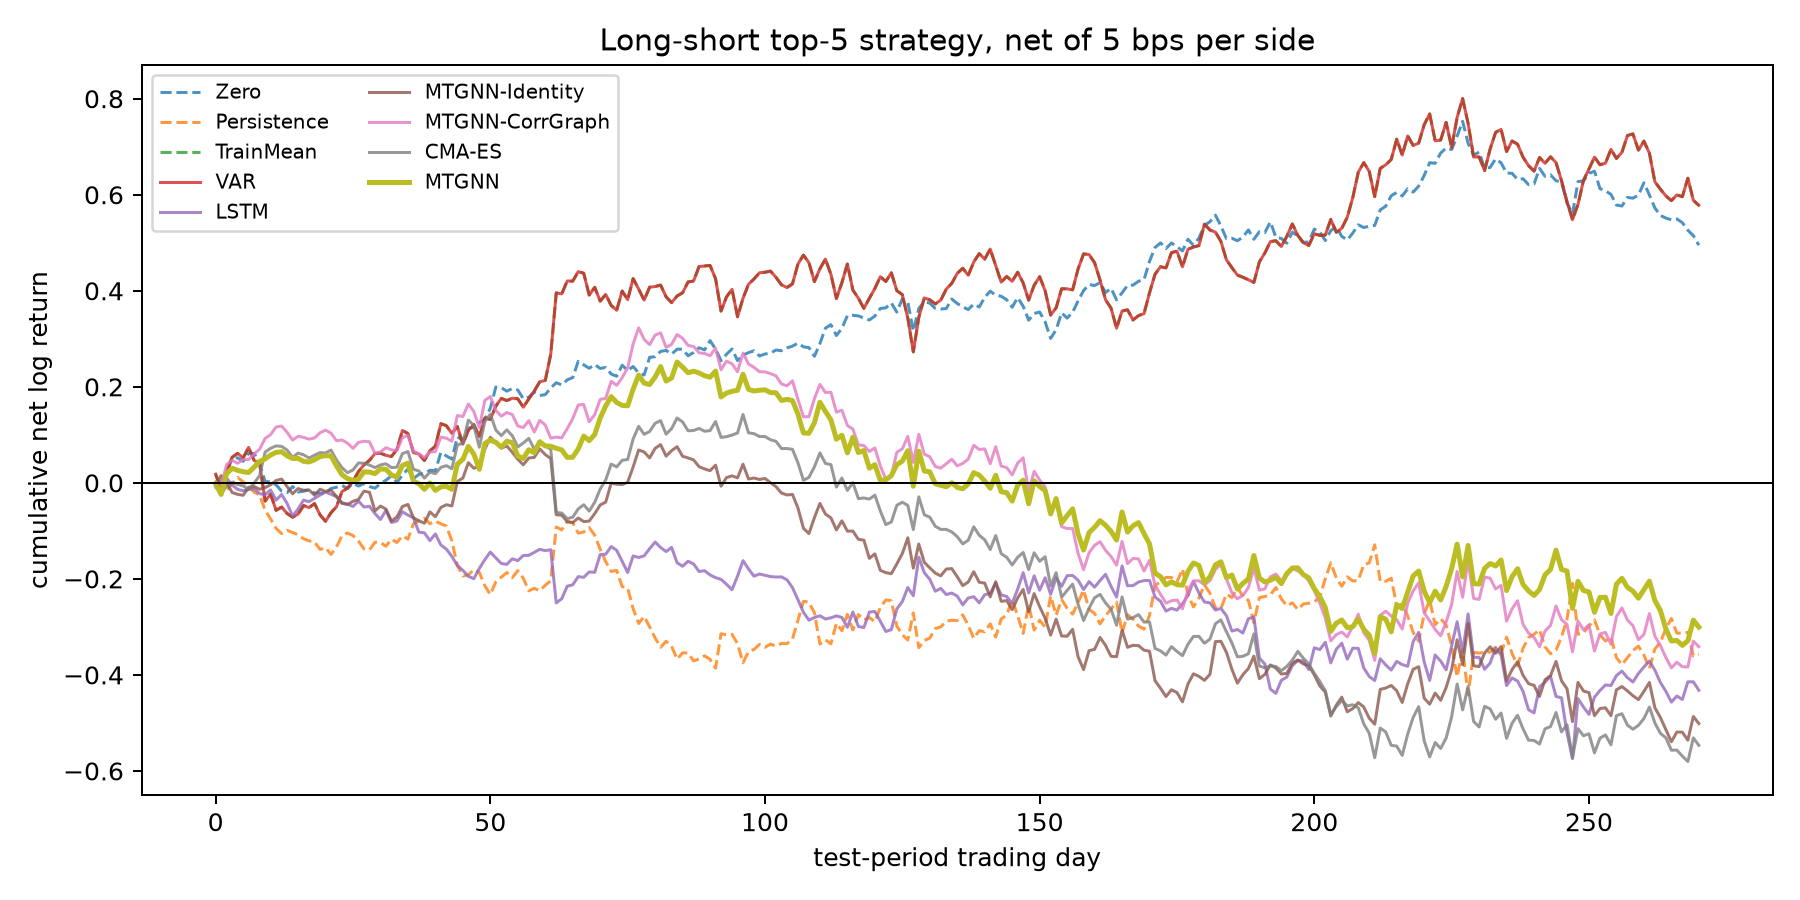
\includegraphics[width=\textwidth]{figures/portfolio.png}
\caption{Cumulative net log return. The two upward curves are the degenerate zero forecast and the constant-basket VAR; both are static bets. Every genuinely time-varying model loses money after costs.}
\label{fig:portfolio}
\end{figure}

Two entries require a caveat more informative than the numbers. The zero forecast posts the best net Sharpe ratio ($1.694$), but its predictions are identical across companies, so the long-short ranking is decided entirely by \texttt{argsort} tie-breaking, that is, by the order companies happen to appear in the data file. We verified its basket is literally constant on all 271 days. Its Sharpe ratio is a property of an arbitrary fixed bet, not of a forecast. VAR's $1.186$ is the same phenomenon in milder form: a constant per-company forecast yields a static basket with turnover $0.007$ against roughly $3.1$ for the time-varying models.

Among models that actually trade, every one has a negative net Sharpe ratio, and turnover explains it. They rebalance the entire book daily, roughly $3.1$ units of turnover, which at 5 bps per side costs about $1.0$ of annualised Sharpe. MTGNN's gross $+0.292$ becomes $-0.679$ net. Transaction costs alone eliminate the gross signal, and that gross signal was not statistically significant to begin with.
